\section{Results}\label{sec:results}
We first report the original MobileFaceNet experiments, followed by the matched encoder replication. Unless stated otherwise, thresholds use a 0.1\% training or validation FAR target, with test FAR measured separately. Rates are expressed as percentages and their differences as percentage points; AUC and cosine similarity are unitless.


Table~\ref{tab:official} reports official-pair verification at a training FAR target of 0.1\%. Protected results average five LFW keys or ten CFP keys. On LFW, matcher-only TAR is 98.66\% for raw embeddings and 82.99\% for 128-bit RO. On CFP-FP, the raw baseline is 87.71\%, while RO TAR is 35.93\% at 128 bits and 80.50\% at 512 bits. The compact 128-bit representation therefore loses much more genuine acceptance in the frontal-to-profile setting.

\begin{table}[t]
\caption{Original MobileFaceNet verification on official pairs.}
\label{tab:official}\centering\small
\begin{tabular}{@{}llrrr@{}}\toprule
Dataset & Representation & TAR (\%) & FAR (\%) & Bytes\\\midrule
LFW & Raw 512-D & 98.66 & 0.101 & 2048\\
LFW & RO 128-bit & 82.99 & 0.094 & 16\\
CFP-FP & Raw 512-D & 87.71 & 0.143 & 2048\\
CFP-FP & RO 64-bit & 14.56 & 0.077 & 8\\
CFP-FP & RO 128-bit & 35.93 & 0.103 & 16\\
CFP-FP & RO 256-bit & 61.49 & 0.129 & 32\\
CFP-FP & RO 512-bit & 80.50 & 0.106 & 64\\\bottomrule
\end{tabular}
\tabnote{Official-pair rates use a 0.1\% training FAR target; LFW results are matcher-only.}
\end{table}

Across the CFP length study, TAR increases from 14.56\% at 64 bits to 80.50\% at 512 bits, leaving a 7.21-percentage-point gap to the raw baseline. The longer representation is consequently included in the attack evaluation: restricting that evaluation to short templates would assess protection at a substantially weaker genuine operating point.

When LFW detection failures count as rejections, full-pipeline TAR is 98.03\% for raw embeddings and 82.47\% for 128-bit RO. These values differ from the matcher-only rates in Table~\ref{tab:official}. CFP uses supplied aligned crops, so complete crop coverage does not demonstrate successful detection on its raw photographs.


Table~\ref{tab:storage} connects template size to the edge motivation. A 128-bit template needs 16 bytes, saving 99.22\% of the raw 2048-byte payload. A 512-bit template needs 64 bytes, saving 96.88\%. Equivalently, the payloads are 128 times and 32 times smaller than the raw embedding. These savings follow directly from the representation sizes and apply to each tested family at the stated length.

\begin{table}[t]
\caption{Packed template payload relative to a raw embedding.}
\label{tab:storage}\centering\small
\begin{tabular}{@{}lrrr@{}}\toprule
Representation & Bytes & Reduction & Saved (\%)\\\midrule
Raw 512-D float32 & 2048 & $1\times$ & 0.00\\
Protected 128-bit & 16 & $128\times$ & 99.22\\
Protected 512-bit & 64 & $32\times$ & 96.88\\\bottomrule
\end{tabular}
\tabnote{Savings cover packed templates only; model, operator, key, and metadata costs are excluded.}
\end{table}

For $N$ enrolled references, the template payload is $2048N$, $16N$, or $64N$ bytes. Increasing CFP RO payload from 16 to 64 bytes raises official TAR from 35.93\% to 80.50\%, but the custom experiments below also reveal greater reconstruction risk. The storage advantage must therefore be weighed against both recognition and exposure outcomes.

Figure~\ref{fig:storage-scaling} expresses the same deterministic payload accounting over database size. It isolates the template component and therefore does not measure full application memory.
\begin{figure}[!tb]
\centering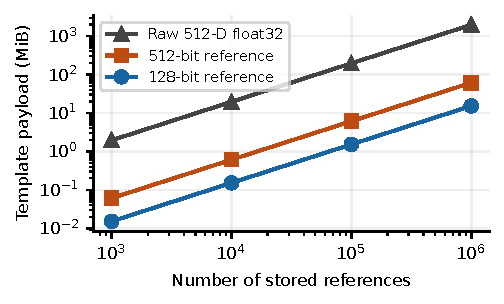
\includegraphics[width=\columnwidth]{storage_scaling.pdf}
\caption{Calculated template-only storage as the number of enrolled references grows. Both axes are logarithmic; one MiB is $2^{20}$ bytes.}
\label{fig:storage-scaling}\fignote{Curves exclude model weights, working memory, keys, operators, and metadata.}
\end{figure}


Table~\ref{tab:replay} tests whether unchanged old bits are accepted after a key change, with version checks bypassed. CFP accepts 106 of 315,000 decisions at 128 bits and 10 at 512 bits. These trials reuse subjects and keys, so the counts describe the test schedule rather than independent risk observations. Recalculation from the cache reproduces the saved scores, thresholds, and decisions.

\begin{table}[t]
\caption{Acceptance of unchanged old templates after renewal.}
\label{tab:replay}\centering\small
\begin{tabular}{@{}lrrr@{}}\toprule
Dataset / bits & Accepted / trials & Rate (\%) & Worst (\%)\\\midrule
LFW / 128 & 28 / 59,620 & 0.04696 & 0.101\\
CFP-FP / 128 & 106 / 315,000 & 0.03365 & 0.2857\\
CFP-FP / 512 & 10 / 315,000 & 0.00317 & 0.0571\\\bottomrule
\end{tabular}
\tabnote{Unchanged old templates rarely pass the renewed matcher; repeated trials are dependent.}
\end{table}

The LFW version gate rejects every revoked version in its test. Genuine acceptance can still vary after renewal: TAR differs by up to 5.64 percentage points between two keys. Basic cross-key Hamming scores give pooled AUC 0.5020 on LFW and 0.5010/0.5027 on CFP at 128/512 bits, close to chance on average. The worst individual key-pair AUC is 0.5256 on LFW and 0.5454 on CFP at 512 bits. The CFP diagnostic compares images without disjoint test-identity partitions and should be read within that scope.


The learned LFW attack finds a small same-person signal. In the original multiple-exposure test, AUC changes from 0.5558 at one exposure to 0.5583 at ten. Rebuilding pairs with separate training and test identities gives 0.5580 and 0.5595. A signal therefore remains for unseen people. Since pair construction also changed, identity separation alone cannot explain the difference between the two tests.

Table~\ref{tab:linkage} gives E06 means for each dataset's own identity-disjoint protocol. With ten exposures, CFP AUC is 0.5323--0.5377 at 128 bits and 0.5629--0.5667 at 512 bits. The longer template improves genuine matching but gives this attacker a stronger ranking signal. Small differences among the projection methods should not be confused with the larger change in threat model when old operators are revealed.

\begin{table}[t]
\caption{Template-only linkage AUC at ten exposures.}
\label{tab:linkage}\centering\small
\begin{tabular}{@{}lrrr@{}}\toprule
Method & LFW 128 & CFP 128 & CFP 512\\\midrule
RO & 0.5594 & 0.5328 & 0.5667\\
SRHT & 0.5577 & 0.5323 & 0.5629\\
PCA-guided RO & 0.5687 & 0.5377 & 0.5643\\\bottomrule
\end{tabular}
\tabnote{AUC describes template-only identity linkage at ten exposures; chance ranking is 0.5.}
\end{table}


Table~\ref{tab:attackutility} gives legitimate utility for the custom E07 protocols at a training/validation FAR target of 0.1\%. In this original custom protocol, the screened CFP raw baseline has TAR 91.47\% and observed FAR 0.325\%. Its images, pair lists, partitions, and thresholds differ from the official benchmark. Attack rates must therefore be compared with this custom protocol's utility, not substituted into the official results.

\begin{table}[t]
\caption{Genuine utility in the original custom attack protocols.}
\label{tab:attackutility}\centering\small
\begin{tabular}{@{}llrr@{}}\toprule
Protocol & Method & TAR (\%) & FAR (\%)\\\midrule
LFW, 128 bits & RO & 83.34 & 0.077\\
 & SRHT & 82.00 & 0.087\\
 & PCA-guided RO & 84.89 & 0.087\\
CFP screened, 128 & RO & 39.33 & 0.134\\
 & SRHT & 37.76 & 0.113\\
 & PCA-guided RO & 43.50 & 0.115\\
CFP screened, 512 & RO & 82.52 & 0.172\\
 & SRHT & 81.95 & 0.167\\
 & PCA-guided RO & 82.38 & 0.200\\\bottomrule
\end{tabular}
\tabnote{These custom-protocol rates are the genuine operating points for the inversion study.}
\end{table}

\begin{table*}[t]
\caption{Original MobileFaceNet calibrated inversion: fresh-key attack success and reconstruction quality.}
\label{tab:inversion}\centering\small
\begin{tabular}{@{}lrlrrrr@{}}\toprule
Protocol & Bits & Method & Fresh ASR, $K=1$ & Fresh ASR, $K=10$ [95\% CI] & Cosine & Raw ASR\\\midrule
% BEGIN GENERATED ATTACK ROWS
LFW & 128 & RO & 9.13 & 66.63 [64.96, 68.31] & 0.8103 & 97.22 \\
LFW & 128 & SRHT & 8.39 & 64.53 [62.86, 66.22] & 0.8096 & 97.30 \\
LFW & 128 & PCA-guided RO & 34.50 & 80.96 [79.47, 82.44] & 0.8635 & 97.53 \\
CFP screened & 128 & RO & 2.01 & 19.66 [17.23, 22.38] & 0.8105 & 84.22 \\
CFP screened & 128 & SRHT & 1.93 & 18.84 [16.42, 21.41] & 0.8099 & 84.28 \\
CFP screened & 128 & PCA-guided RO & 7.86 & 32.94 [29.35, 36.96] & 0.8593 & 86.32 \\
CFP screened & 512 & RO & 63.27 & 78.02 [73.38, 82.52] & 0.9725 & 88.22 \\
CFP screened & 512 & SRHT & 62.64 & 77.52 [72.95, 82.10] & 0.9726 & 88.09 \\
CFP screened & 512 & PCA-guided RO & 70.28 & 78.54 [73.89, 83.03] & 0.9809 & 88.72 \\
% END GENERATED ATTACK ROWS

\bottomrule
\end{tabular}
\tabnote{ASR values are percentages; brackets show conditional 95\% intervals for fresh-key ASR at ten exposures.}
\end{table*}

\begin{figure*}[!t]
\centering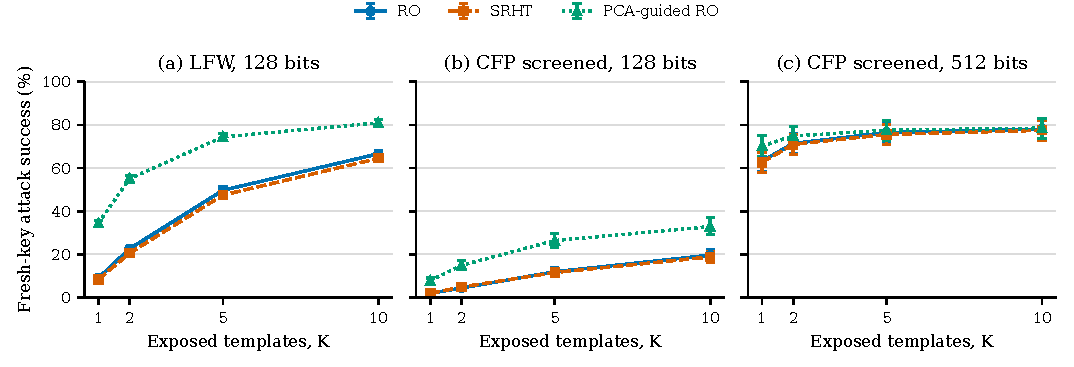
\includegraphics[width=\textwidth]{exposure.pdf}
\caption{Fresh-key attack success increases with exposure; error bars show conditional 95\% identity-bootstrap intervals.}
\label{fig:exposure}
\fignote{More exposed records provide useful reconstruction information in the tested configurations.}
\end{figure*}

\begin{figure*}[!t]
\centering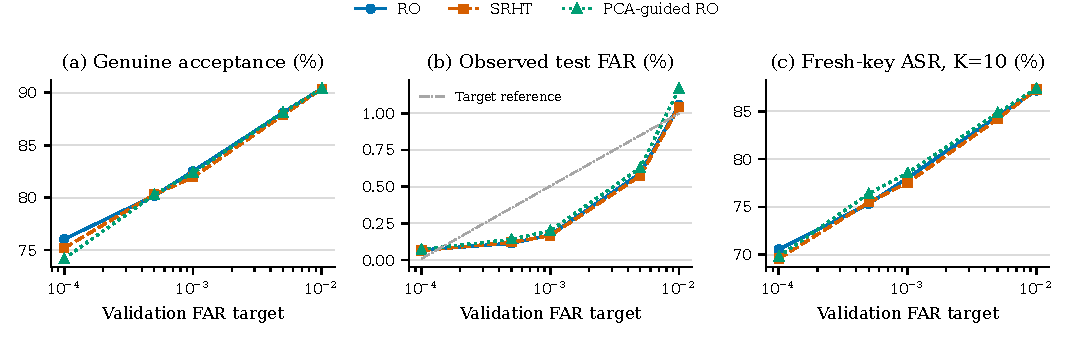
\includegraphics[width=\textwidth]{thresholds.pdf}
\caption{Stricter validation targets reduce genuine and attack acceptance on screened CFP at 512 bits.}
\label{fig:thresholds}
\fignote{Lower attack acceptance must be interpreted together with genuine-user rejection.}
\end{figure*}

Across the three projection methods, calibrated cross-image fresh-key ASR at ten exposures is 64.53--80.96\% on LFW at 128 bits, 18.84--32.94\% on screened CFP at 128 bits, and 77.52--78.54\% on screened CFP at 512 bits. The CFP attack pool contains 5704 crops from 500 identities before partitioning. These ranges describe the original run; the matched CFP encoder replication is reported separately below. Table~\ref{tab:inversion} reports ASR in percent; its brackets give conditional 95\% identity-bootstrap intervals from 2000 replicates. Cosine similarity and raw ASR are measured at $K=10$, with cosine taken against the exposed image.

Figure~\ref{fig:exposure} shows the exposure effect on a common vertical scale. In both result figures, blue solid lines with circles represent RO, orange dashed lines with squares represent SRHT, and green dotted lines with triangles represent PCA-guided RO. Exposure error bars show pointwise conditional 95\% intervals. LFW and CFP retain their separate protocols.

On LFW, ten-exposure ASR is 66.63\% for RO, 64.53\% for SRHT, and 80.96\% for PCA-guided RO. The corresponding uninformed rates are 0.53\%, 0.40\%, and 0.13\%. Acceptance against the exposed image is almost 100\%. Testing against a different photograph is therefore a more informative primary measure than reusing the source image.

At 128 bits on CFP, RO and SRHT recover the source embedding with cosine similarities 0.8105 and 0.8099, close to LFW's 0.8103 and 0.8096. Yet fresh-key cross-pose ASR is only 19.66\% and 18.84\%. PCA-guided RO gives cosine 0.8593 and ASR 32.94\%. This lower attack acceptance accompanies weak genuine cross-pose recognition. Under the separate raw-matcher threshold, reconstructed CFP embeddings reach 84.22--86.32\% ASR.

At 512 bits on CFP, cosine similarity reaches 0.9725, 0.9726, and 0.9809 for RO, SRHT, and PCA-guided RO. Their fresh-key ASRs are 78.02\% [73.38, 82.52], 77.52\% [72.95, 82.10], and 78.54\% [73.89, 83.03]. Uninformed rates are 0.08--0.16\%, while raw ASR is 88.09--88.72\%. The rare acceptance of unchanged old bits does not account for these newly reconstructed inputs.

Diagonal calibration is not necessary for substantial acceptance in the 512-bit CFP setting. At ten exposures, analytical backprojection reaches ASRs of 77.93\%, 77.33\%, and 78.06\% for RO, SRHT, and PCA-guided RO, respectively. Calibration provides only a small additional gain here. These results establish the measured risk with a simple estimator; they do not assess what a more complex decoder might recover.


All paired intervals for calibrated $K=10$ minus $K=1$ ASR lie above zero. The increases for RO, SRHT, and PCA-guided RO are 57.50, 56.13, and 46.46 percentage points on LFW; 17.64, 16.91, and 25.09 on CFP at 128 bits; and 14.76, 14.88, and 8.27 on CFP at 512 bits. The 512-bit increases are smaller because single-exposure ASR is already 62.64--70.28\%.

At ten exposures, the CFP 512-bit intervals overlap across methods. The source package includes paired method contrasts, but ranking protection from the point estimates alone is not justified. Under known-operator exposure, substantial attack acceptance occurs for all three projection families.


Figure~\ref{fig:thresholds} reports means over fixed keys and splits for screened CFP at 512 bits. The attack panel uses calibrated reconstruction with ten exposures. The gray dash-dot line in the FAR panel marks equality between test FAR and the validation target, expressed as percentages. For RO, tightening the target from $10^{-3}$ to $10^{-4}$ lowers TAR from 82.52\% to 76.04\% and ASR from 78.02\% to 70.56\%. Across methods, ASR remains 69.59--70.56\% at the tighter setting. At the looser $10^{-2}$ target, TAR is about 90.4\% and ASR is 87.17--87.38\%. Stricter matching reduces acceptance for both users and attackers but does not remove the observed risk.

Each validation split contains only 2105--2173 impostor comparisons. The $10^{-4}$ target allows no validation false accepts, yet test FAR is 0.0656--0.0736\%, above the nominal 0.01\%. This sample cannot establish a population FAR of $10^{-4}$. At the main 0.1\% target, CFP 512-bit test FAR is 0.167--0.200\%. Every operating point must therefore be interpreted with its observed FAR.




On official CFP-FP pairs, raw TAR increases from 87.71\% for MobileFaceNet to 94.89\% for ResNet50 at the 0.1\% training-FAR target. Both have observed test FAR 0.143\%. Table~\ref{tab:encoder-cfp} reports the separate screened-subset comparison. Protected TAR rises for every method and length: from \MbfSmallTar{} to \RnetSmallTar{} at 128 bits, and from \MbfLargeTar{} to \RnetLargeTar{} at 512 bits.

Higher utility does not remove the tested reconstruction vulnerability. At ten exposures, MobileFaceNet calibrated cross-image fresh-key ASR is \MbfSmallAsr{} at 128 bits and \MbfLargeAsr{} at 512 bits. The corresponding ResNet50 ranges are \RnetSmallAsr{} and \RnetLargeAsr{}. All six paired ResNet50-minus-MobileFaceNet ASR intervals lie above zero. These pointwise intervals resample the 195 unique test identities while retaining dependencies across overlapping splits and keys; they condition on the fitted models and thresholds. They do not establish that every stronger encoder is less secure.

Fresh-key acceptance and reconstruction cosine do not improve in parallel. For 128-bit RO and SRHT, exposed-image cosine stays near 0.81 with either encoder, although acceptance rises with ResNet50. All three 512-bit ResNet50 configurations also admit high acceptance. Thus, stronger genuine recognition cannot be taken as evidence that the protected representation better resists known-operator reconstruction.

Table~\ref{tab:encoder-lfw} gives the corresponding LFW recognition extension. Raw matcher-only TAR changes from 98.66\% to 99.03\%. At 128 bits, ResNet50 TAR is 92.28\% for RO, 92.10\% for SRHT, and 94.66\% for PCA-guided RO, compared with 82.99\%, 84.48\%, and 85.22\% for MobileFaceNet. These recognition results extend the utility comparison; they do not extend the LFW attack evidence.

\begin{table*}[t]
\caption{Matched encoder comparison on screened CFP. Rates are percentages; ASR differences are percentage points.}
\label{tab:encoder-cfp}\centering\footnotesize
\begin{tabular}{@{}rlrrrrr@{}}\toprule
Bits & Method & MBF TAR / FAR & R50 TAR / FAR & MBF ASR & R50 ASR & ASR difference [95\% CI]\\\midrule
128 & RO & 39.33 / 0.134 & 65.50 / 0.133 & 19.66 & 38.46 & 18.80 [16.68, 20.86]\\
128 & SRHT & 37.76 / 0.113 & 65.12 / 0.120 & 18.84 & 38.28 & 19.43 [17.03, 21.81]\\
128 & PCA-guided RO & 43.50 / 0.115 & 66.94 / 0.103 & 32.96 & 53.09 & 20.13 [17.74, 22.68]\\
512 & RO & 82.52 / 0.172 & 94.61 / 0.134 & 78.02 & 92.30 & 14.28 [11.13, 17.52]\\
512 & SRHT & 81.95 / 0.167 & 94.67 / 0.128 & 77.52 & 92.23 & 14.71 [11.67, 17.95]\\
512 & PCA-guided RO & 82.38 / 0.200 & 94.37 / 0.130 & 78.56 & 92.03 & 13.48 [10.34, 16.72]\\
\bottomrule\end{tabular}
\tabnote{MBF: MobileFaceNet; R50: ResNet50 ArcFace. Each encoder has a separate validation-only threshold targeting 0.1\% FAR. ASR is calibrated cross-image fresh-key acceptance at $K=10$. The fresh operator is hidden from reconstruction. Paired percentile intervals use 2000 identity resamples and condition on the fitted pipelines; they are pointwise and not multiplicity-adjusted. These replication runs remain separate from the original baseline tables.}
\end{table*}

\begin{table}[t]
\centering
\caption{LFW official-pair recognition: encoder comparison.}
\label{tab:encoder-lfw}
\small
\begin{tabular}{lrrrr}
\toprule
& \multicolumn{2}{c}{TAR (\%)} & \multicolumn{2}{c}{FAR (\%)} \\
Method & MBF & R50 & MBF & R50 \\
\midrule
Raw & 98.66 & 99.03 & 0.101 & 0.101 \\
RO & 82.99 & 92.28 & 0.094 & 0.080 \\
SRHT & 84.48 & 92.10 & 0.094 & 0.094 \\
PCA-guided RO & 85.22 & 94.66 & 0.087 & 0.094 \\
\bottomrule
\end{tabular}
\tabnote{Matcher-only evaluation uses 5965 valid pairs, with thresholds fitted on the other nine folds at a 0.1\% FAR target. Protected templates have 128 bits; rates average five fixed keys. MBF: MobileFaceNet; R50: ResNet50 ArcFace. The full 6000-pair operational results are retained in the evidence. Fold-specific PCA excludes held-out identities from fitting.}
\end{table}


\begin{figure*}[!t]
\centering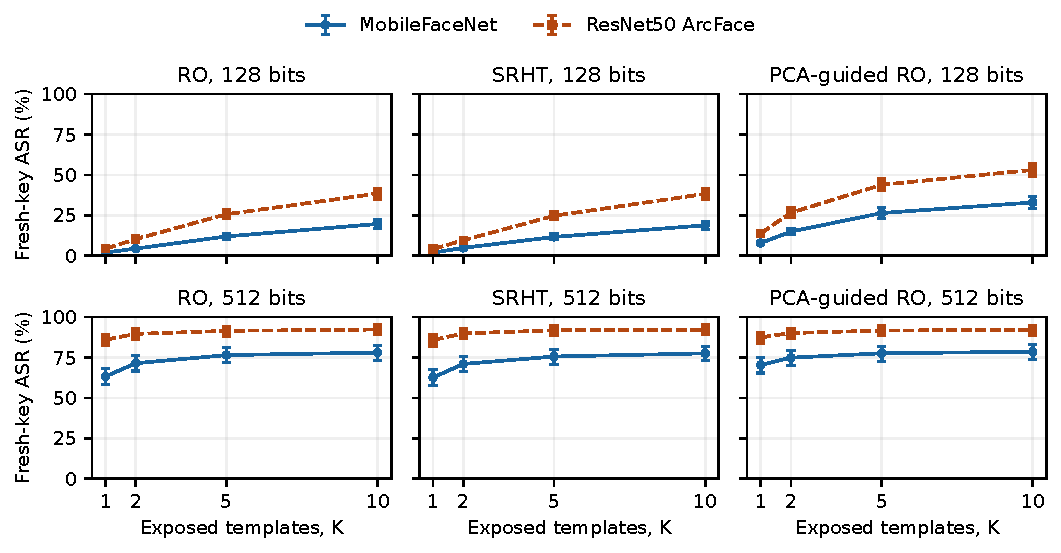
\includegraphics[width=0.92\textwidth]{encoder_exposure.pdf}
\caption{CFP encoder replication: calibrated cross-image fresh-key ASR over exposure count at 128 bits (top) and 512 bits (bottom). Error bars show pointwise conditional 95\% identity-bootstrap intervals. Both encoders use identical screened crops and exposure schedules, with separately fitted models and validation-only thresholds.}
\label{fig:encoder-exposure}
\fignote{The stronger recognition checkpoint still permits substantial fresh-key attack acceptance.}
\end{figure*}


Unchanged old CFP records continue to have low cross-image replay acceptance. Across the two encoders, three methods, and two directions, mean transition rates are approximately 0.038--0.076\% at 128 bits and 0.004--0.013\% at 512 bits. Template-only linkage with ten records has trained-score AUC 0.530--0.542 at 128 bits and 0.559--0.567 at 512 bits. These descriptive outcomes concern the tested classifier and fixed key schedule; they do not prove unlinkability or resistance to a stronger attacker.

The replication reports conditional intervals at validation-FAR targets $10^{-4}$, $10^{-3}$, and $10^{-2}$, together with a descriptive threshold sweep and measured test FAR alongside TAR and ASR. Complete exposure curves, paired contrasts, and threshold plots are retained in the accompanying results. Lower attack acceptance under stricter matching must be read alongside increased genuine rejection. The hidden fresh operator and digital embedding-input interface remain unchanged.


Figures~\ref{fig:cfp-recognition} and~\ref{fig:lfw-recognition} present recognition separately for the screened CFP protocol and official LFW pairs. CFP intervals quantify conditional identity variation; LFW error bars describe variation across five fixed keys and are not confidence intervals. The two uncertainty summaries must not be conflated.

Figure~\ref{fig:paired-encoder} reports paired differences directly. At the primary validation target, all six protected-recognition contrasts and all six calibrated ten-exposure ASR contrasts favor higher acceptance with ResNet50. Figure~\ref{fig:paired-exposure} shows that all twelve calibrated exposure-growth intervals are positive. These pointwise results quantify consistency across the tested configurations without providing simultaneous family-wise coverage.

Figure~\ref{fig:reconstruction-quality} distinguishes recovery of the exposed image's embedding from transfer to a different photograph of the same identity. These endpoints capture source fidelity and cross-image identity information, respectively. Neither substitutes for the fresh-key acceptance test, whose outcome also depends on the transformation and threshold.

\begin{figure}[!tb]
\centering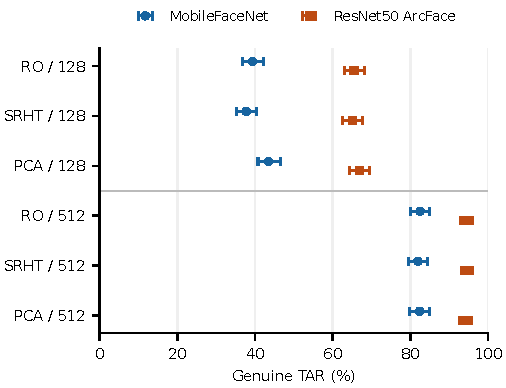
\includegraphics[width=\columnwidth]{cfp_recognition_ci.pdf}
\caption{Protected genuine recognition on screened CFP at the $10^{-3}$ validation-FAR target. Error bars are pointwise conditional 95\% identity-bootstrap intervals.}
\label{fig:cfp-recognition}\fignote{Matched inputs and protocols use encoder-specific fits and thresholds; PCA denotes PCA-guided RO, and row suffixes give bit lengths.}
\end{figure}
\begin{figure}[!tb]
\centering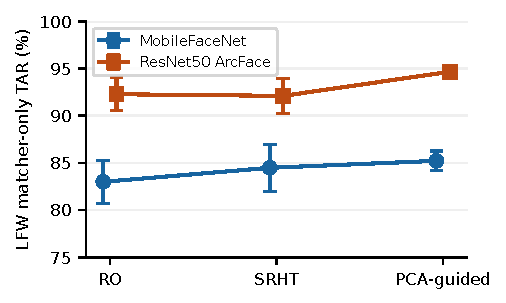
\includegraphics[width=\columnwidth]{lfw_recognition_sd.pdf}
\caption{LFW matcher-only recognition at 128 bits under official folds. Error bars show one standard deviation across five keys, not confidence intervals.}
\label{fig:lfw-recognition}\fignote{This extension evaluates recognition; it does not provide a second-encoder LFW attack result.}
\end{figure}
\begin{figure}[!tb]
\centering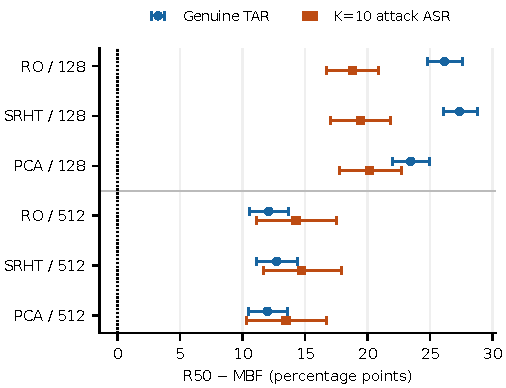
\includegraphics[width=\columnwidth]{paired_encoder_effects.pdf}
\caption{Paired ResNet50-minus-MobileFaceNet differences in genuine TAR and calibrated fresh-key ASR at $K=10$. Bars show pointwise conditional 95\% intervals; the dotted line marks zero.}
\label{fig:paired-encoder}\fignote{Positive differences mean higher acceptance, which has different implications for genuine and attack inputs.}
\end{figure}
\begin{figure}[!tb]
\centering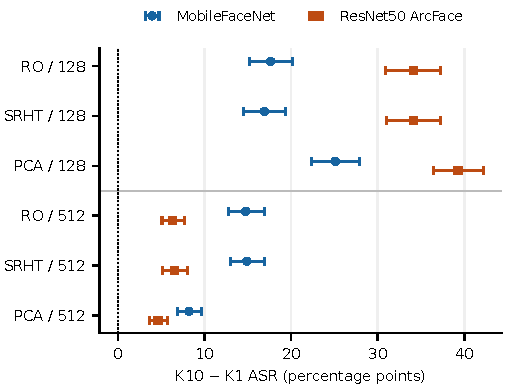
\includegraphics[width=\columnwidth]{paired_exposure_effects.pdf}
\caption{Paired $K=10$ minus $K=1$ calibrated fresh-key ASR differences for screened CFP. Bars show pointwise conditional 95\% intervals at the $10^{-3}$ validation-FAR target.}
\label{fig:paired-exposure}\fignote{Every plotted interval lies above zero; trials sharing an identity retain common bootstrap weights.}
\end{figure}
\begin{figure*}[!t]
\centering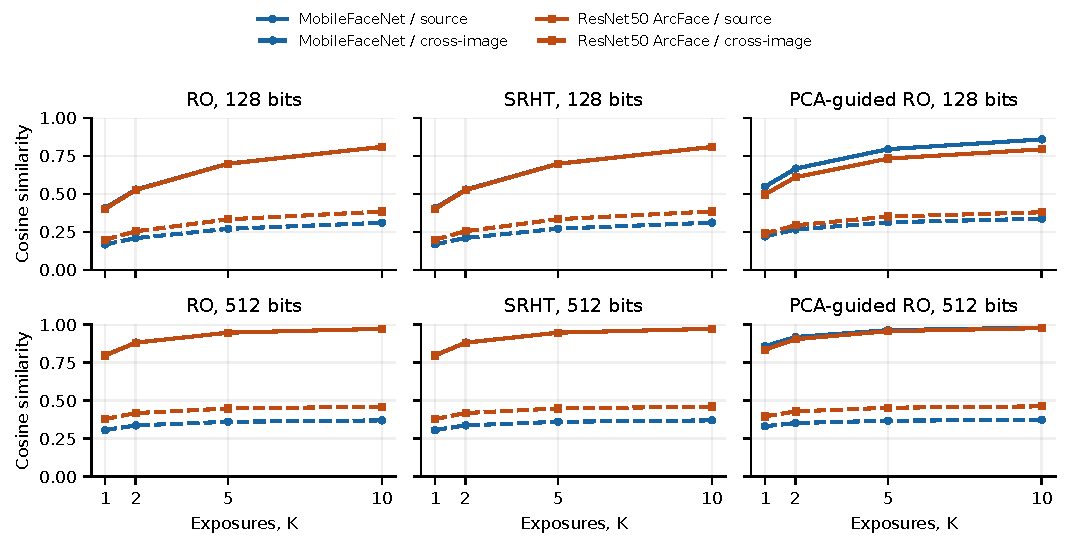
\includegraphics[width=.97\textwidth]{reconstruction_quality.pdf}
\caption{Calibrated reconstruction cosine over exposure count on screened CFP. Color identifies the encoder; solid and dashed lines distinguish the exposed source from the cross-image reference.}
\label{fig:reconstruction-quality}\fignote{Lines show point estimates, not uncertainty bands; cosine is unitless and is not attack acceptance.}
\end{figure*}
\begin{figure}[!tb]
\centering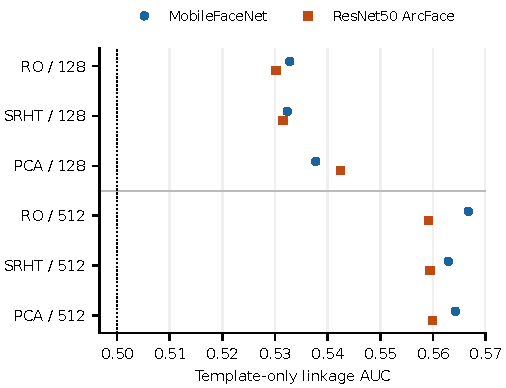
\includegraphics[width=\columnwidth]{linkage_comparison.pdf}
\caption{Template-only linkage at $K=10$ in the matched CFP replication. The dotted line denotes chance AUC; these descriptive means have no added confidence intervals.}
\label{fig:linkage-enc}\fignote{The learned score shows limited discrimination under this access model, which excludes old operators.}
\end{figure}

Figure~\ref{fig:linkage-enc} complements the inversion results with the template-only attacker. Figures~\ref{fig:enc-target128} and~\ref{fig:enc-target512} show how validation targets alter genuine acceptance, test FAR, and attack acceptance. At target $10^{-4}$, calibrated 512-bit $K=10$ ASR remains 69.59--70.54\% for MobileFaceNet and 89.01--90.09\% for ResNet50. These values belong to the matched replication, distinct from the original MobileFaceNet sweep. The stricter target reduces attack acceptance without demonstrating population FAR control at $10^{-4}$.
\begin{figure*}[!t]
\centering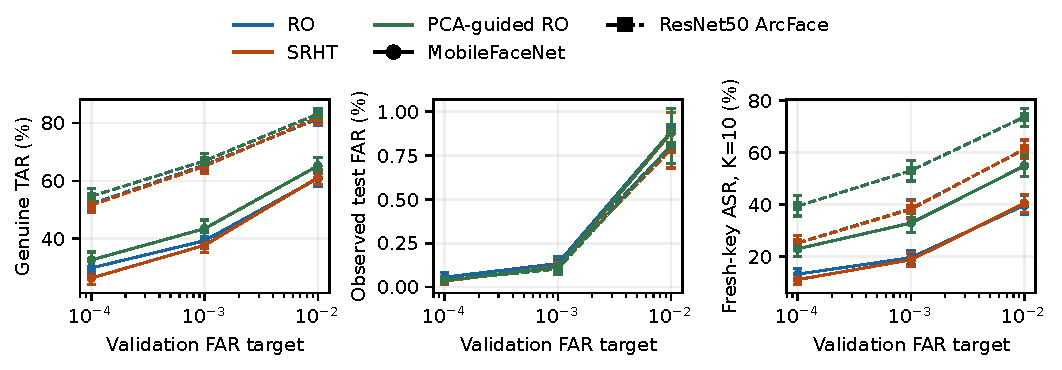
\includegraphics[width=\textwidth]{encoder_threshold_targets_128.pdf}
\caption{Matched CFP sensitivity at 128 bits: genuine TAR, observed test FAR, and calibrated $K=10$ fresh-key ASR at three validation-FAR targets. Error bars show pointwise conditional 95\% intervals.}
\label{fig:enc-target128}\fignote{Validation targets set the thresholds; the middle panel reports the separately observed test FAR.}
\end{figure*}
\begin{figure*}[!t]
\centering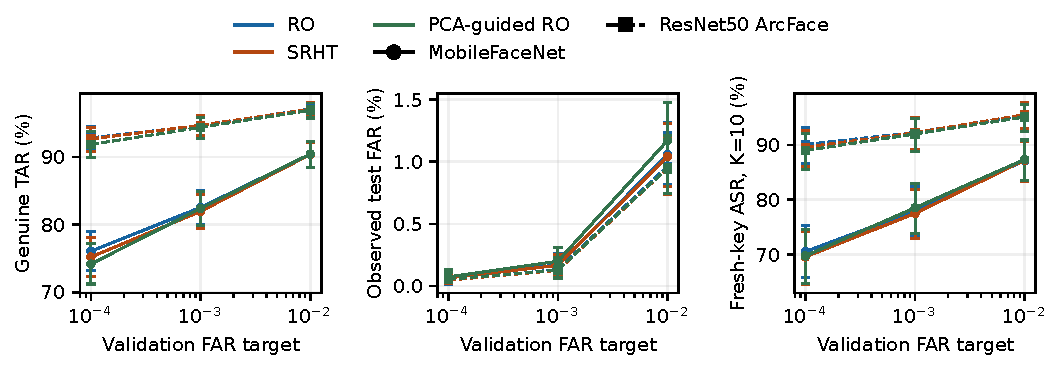
\includegraphics[width=\textwidth]{encoder_threshold_targets_512.pdf}
\caption{Matched CFP sensitivity at 512 bits with the same endpoints and validation-target convention as Fig.~\ref{fig:enc-target128}. Error bars show pointwise conditional 95\% intervals.}
\label{fig:enc-target512}\fignote{Substantial attack acceptance persists at the strictest evaluated validation target.}
\end{figure*}

